\documentclass[11pt, oneside]{article}   	% use "amsart" instead of "article" for AMSLaTeX format
\usepackage[margin=1in]{geometry}                		% See geometry.pdf to learn the layout options. There are lots.
\geometry{letterpaper}                   		% ... or a4paper or a5paper or ... 
%\geometry{landscape}                		% Activate for rotated page geometry
%\usepackage[parfill]{parskip}    		% Activate to begin paragraphs with an empty line rather than an indent
\usepackage{graphicx}				% Use pdf, png, jpg, or eps§ with pdflatex; use eps in DVI mode
								% TeX will automatically convert eps --> pdf in pdflatex		
\usepackage{amssymb}
%usepackage{undertilde}
\usepackage[numbered,framed]{matlab-prettifier}

\usepackage[T1]{fontenc}
\usepackage{mathtools}  % loads »amsmath«
\usepackage{physics}
\usepackage{listings}

\lstset{
  language=C,                % choose the language of the code
  numbers=left,                   % where to put the line-numbers
  stepnumber=1,                   % the step between two line-numbers.        
  numbersep=5pt,                  % how far the line-numbers are from the code
  backgroundcolor=\color{white},  % choose the background color. You must add \usepackage{color}
  showspaces=false,               % show spaces adding particular underscores
  showstringspaces=false,         % underline spaces within strings
  showtabs=false,                 % show tabs within strings adding particular underscores
  tabsize=2,                      % sets default tabsize to 2 spaces
  captionpos=b,                   % sets the caption-position to bottom
  breaklines=true,                % sets automatic line breaking
  breakatwhitespace=true,         % sets if automatic breaks should only happen at whitespace
  title=\lstname,                 % show the filename of files included with \lstinputlisting;
}

\setlength{\parskip}{0.5em}

%SetFonts
\newcommand\Rey{\mbox{\textit{Re}}}

\title{\vspace{-6ex}\large PHYS 516: Methods of Computational Physics \\
  \normalsize ASSIGNMENT 3- MC Simulation of the Ising Model}
\author{Anup V Kanale}
\date{\vspace{-3ex}\today}							% Activate to display a given date or no date

\begin{document}
\maketitle
\section{Theoretical Foundation of Metropolis Algorithm}
Consider a set of N states, {$\Gamma_1, \Gamma_2, ..., \Gamma_N$} and let the probability to find the system in the $m$-th state, $\Gamma_m$, be $\rho_m$. Here, we prove that the probability distribution is a fixed point of the metropolis transition matrix defined below, i.e., $\Pi \rho = \rho$.

\[
\text{(Metropolis transition matrix)} \pi_{mn}= 
\begin{dcases}
	\alpha_{mn} & \rho_m \geq \rho_n m \neq n \\
    \frac{\rho_m}{rho_n} \alpha_{mn} & \rho_m \leq \rho_n m \neq n \\
    1- \sum\limits_{m' \neq n} \pi_{m'n}
\end{dcases}
\]

Here, $\pi_{mn}$ are elements of the matrix $\Pi$, $\rho_m$ are the elements of vector $\rho$, and $\alpha_{mn}$ are elements of a symmetric attempt matrix, i.e., $\alpha_{mn}= \alpha_{nm}$.

This can be proved by enforcing the Detailed Balance condition. Consider a pair of states $m$ and $n$. Assuming $\rho_m < \rho_n$, 
	\begin{equation}
	\pi_{nm} \rho_m = \alpha_{nm} \rho_m = \alpha_{mn} \rho_m
	\end{equation}
where the second equality holds because of the symmetric attempt.
For the same case,
	\begin{equation}
	\pi_{mn} \rho_n = \frac{\rho_m}{\rho_n} \alpha_{mn} \rho_n = \alpha_{mn} \rho_m
	\end{equation}
Using equations 1 and 2,
	\begin{equation}
	\pi_{nm} \rho_m = \pi_{mn} \rho_n
	\end{equation}
The left-hand side is a flux of probability that the current state is $n$ and that the next state is $m$, and the right-hand side is a flux from $m$ to $n$.

In order to show that above detailed balance condition is sufficient for the unit-eigenvalue relation, sum
the both side over n.
	\begin{align}
	\sum\limits_{n=1}^{N} \pi_{mn} \rho_n &= \underbrace{\sum\limits_{n=1}^{N} \pi_{nm}}_{=1} \rho_m \\
	\implies \sum\limits_{n=1}^{N} \pi_{mn} \rho_n &= \rho_m \\
	\therefore \Pi \rho &= \rho
	\end{align}
	
\section{2D Ising Model}
Ising model is used for modelling ferromagnetic materials. This model represents a lattice consisting of atoms which have quantum mechanical spin, which can be $ \pm 1$. When these individual magnetic fields are aligned in the same direction, it gives rise to macroscopic magnetic field. This strong alignment arises from exchange interactions between electrons.

\vspace{-2ex} \subsection{Computer Simulation}
\vspace{-2ex} A program was written  in C to simulate the 2D Ising model.
\lstinputlisting[language=C, frame=single]{IsingModel.c}

\subsection{Results}
The plots below show the Mean magnetization and its standard deviation as a function of the exchange coupling, and a histogram showing the number of MC samples for every value of Magnetization.
	\begin{figure} [!htbp]
	 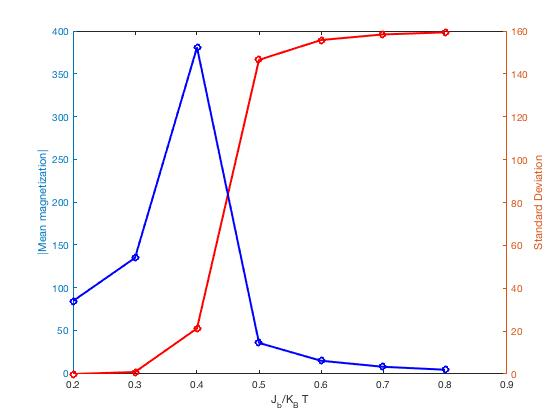
\includegraphics[scale=0.43]{Magn_SD_plot.jpg}
	 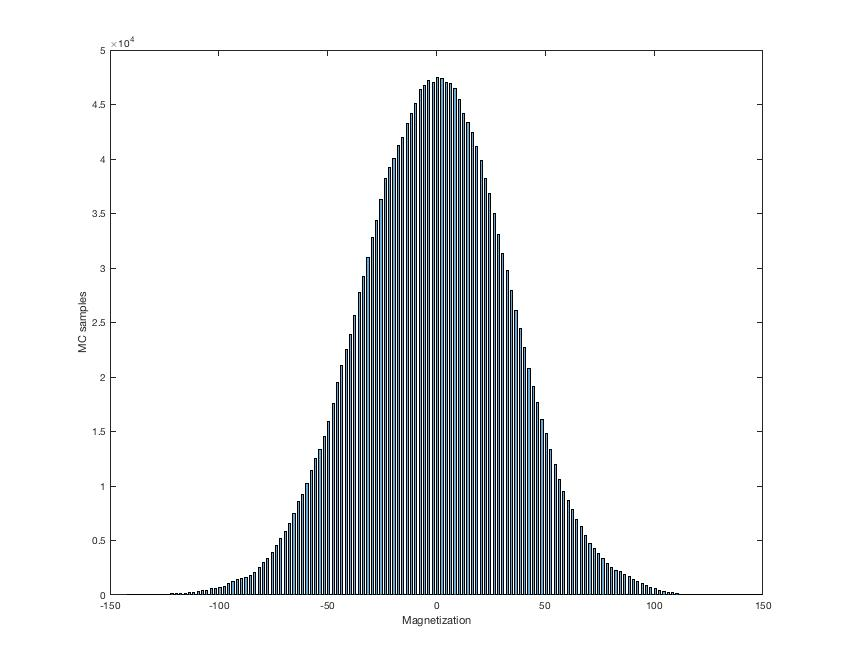
\includegraphics[scale=0.28]{histogram.jpg}
	\caption{Plot of Magnetization and S.D vs $J/K_B T$, and Histogram for $J/K_B T = 0.2$}
	\end{figure}
The matlab script used to generate these plots is shown below.
	\lstinputlisting[style=Matlab-editor]{Ising_MagnetizationPlots.m}
\end{document}